\section{Trigonometric Substitution} \label{S:5.3.TrigSub}

\begin{goals}
\item What techniques should we use when encountering integras involving expressions containing $\sqrt{a^2-x^2}$, $\sqrt{a^2+x^2}$ and $\sqrt{x^2-a^2}$?
\end{goals}

%-----------------------------------
%SUBSECTION: INTRODUCTION
%-----------------------------------
\subsection*{Introduction}

In Section~\ref{S:4.3.DefiniteIntegral} we defined the definite integral as the ``signed area under the curve.'' In that section we had not yet learned the Fundamental Theorem of Calculus, so we evaluated special definite integrals which described nice, geometric shapes. For instance, we were able to evaluate
\begin{equation}
\int_{-3}^3\sqrt{9-x^2}\ dx = \frac{9\pi}{2}\label{eq:trigsub1}
\end{equation}
 as we recognized that $f(x) = \sqrt{9-x^2}$ described the upper half of a circle with radius $3$. 
 
 We have since learned a number of integration techniques, including Substitution and Integration by Parts, yet we are still unable to evaluate the above integral without resorting to a geometric interpretation. This section introduces Trigonometric Substitution, a method of integration that fills this gap in our integration skill. This technique works on the same principle as Substitution as found in Section~\ref{S:4.6.Substitution}, though it can feel ``backward.'' In Section~\ref{S:4.6.Substitution}, we set $u=f(x)$, for some function $f$, and replaced $f(x)$ with $u$. In this section, we will set $x=f(\theta)$, where $f$ is a trigonometric function, then replace $x$ with $f(\theta)$. 


\begin{pa} \label{PA:5.3}
In Section~\ref{S:2.8.Inverse}, we discussed derivatives of inverse functions including the inverse trigonometric functions $\arcsin (x)$, $\arccos (x)$, and $\arctan (x)$. We will need the techniques to find the derivatives to evaluate integrals of a certain form. Let's review the technique.
Suppose $f(x) = \arcsin (x)$ for $-1<x<1$ and $g(x)=\arctan(x)$ for $-1<x<1$
	\be
		\item Rewrite $f(x)$ as $\theta$. Label the right triangle that corresponds to $\theta=\arcsin(x)$. 
		\item Use the completed triangle to show $$ \tan (\arcsin (x)) = \frac{x}{1-x^2} $$
		\item Rewrite $g(x)$ as $\phi$. Label the right triangle that corresponds to $\phi=\arctan(x)$.
		\item Use the completed triangle to show $$ \cos (\arctan (x)) = \frac{1}{\sqrt{1+x^2}} $$
	\ee
\end{pa} 
\afterpa

%add two triangles like figure 2.41 % PREVIEW 

%-----------------------------------------------------------
% SUBSECTION TRIGONOMETRIC SUBSTITUTION
%-----------------------------------------------------------
\subsection*{Trigonometric Substitution}

We now describe in detail Trigonometric Substitution. This \newline method excels when dealing with integrands that contain \newline $\sqrt{a^2-x^2}$, $\sqrt{x^2-a^2}$ and $\sqrt{x^2+a^2}$. The following Concept outlines the procedure for each case.

\concept{Trigonometric Substitution} % CONCEPT
{\begin{enumerate}[1)]
\item For integrands containing $\sqrt{a^2-x^2}$:\index{integration!trig. subst.} \label{C.5.3-sin}\\[5pt]
	Let $x=a\sin(\theta)$, and $dx = a\cos(\theta)\ d\theta$\\[5pt]	
	Thus $\theta = \arcsin(x/a)$, for $-\pi/2\leq \theta\leq \pi/2$. \\[5pt]	
	On this interval, $\cos(\theta)\geq 0$, so\\[5pt]	
	$\sqrt{a^2-x^2} = a\cos(\theta)$.
		
\item For integrands containing $\sqrt{x^2+a^2}$: \label{C.5.3-tan} \\[5pt]
	Let $x=a\tan(\theta)$, and $dx = a\sec^2(\theta)\ d\theta$\\[5pt]	
	Thus $\theta = \arctan(x/a)$, for $-\pi/2 < \theta < \pi/2$. \\[5pt]	
	On this interval, $\sec(\theta)> 0$, so\\[5pt]	
	$\sqrt{x^2+a^2} = a\sec(\theta)$.
		
\item For integrands containing $\sqrt{x^2-a^2}$: \label{C.5.3-sec} \\[5pt]
	Let $x=a\sec(\theta)$, and $dx = a\sec(\theta)\tan(\theta)\ d\theta$\\[5pt]	
	Thus $\theta = \arcsec(x/a)$. If $x/a\geq 1$, then $0\leq\theta<\pi/2$; if $x/a \leq -1$, then $\pi/2<\theta\leq \pi$.\\[5pt]	
	We restrict our work to where $x\geq a$, so $x/a\geq 1$, and $0\leq\theta<\pi/2$.
	On this interval, $\tan(\theta)\geq 0$, so\\[5pt]	
	$\sqrt{x^2-a^2} = a\tan(\theta)$.
\end{enumerate}
} % end concept

\begin{marginfigure}[-12cm] % MARGIN FIGURE
\subfloat[For integrands containing $\sqrt{a^2-x^2}$.]{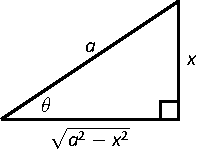
\includegraphics[scale=1.25]{figures/figtrigsub_intro1}}

\subfloat[For integrands containing $\sqrt{x^2+a^2}$.]{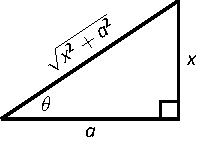
\includegraphics[scale=1.25]{figures/figtrigsub_intro3}}

\subfloat[For integrands containing $\sqrt{x^2-a^2}$.]{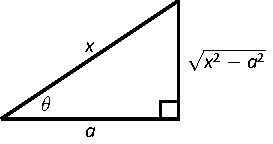
\includegraphics[scale=1.25]{figures/figtrigsub_intro2}}
\caption{The right triangles that correspond to the various trigonometric substitutions.}
\label{fig:trigsub}
\end{marginfigure}

\begin{example} \label{eg:5.3.1} % EXAMPLE
Evaluate $\ds \int_{-3}^3\sqrt{9-x^2}\ dx$.

\solution We begin by noting that $9\sin^2(\theta) + 9\cos^2(\theta) = 9$, and hence $9\cos^2(\theta) = 9-9\sin^2(\theta)$. If we let $x=3\sin(\theta)$, then $9-x^2 = 9-9\sin^2(\theta) = 9\cos^2(\theta)$. 

Setting $x=3\sin(\theta)$ gives  $dx = 3\cos(\theta)\ d\theta$. We are almost ready to substitute. We also wish to change our bounds of integration. The bound $x=-3$ corresponds to $\theta = -\pi/2$ (for when $\theta = -\pi/2$, $x=3\sin(\theta) = -3$). Likewise, the bound of $x=3$ is replaced by the bound $\theta = \pi/2$. Thus
\begin{align*}
\int_{-3}^3\sqrt{9-x^2}\ dx &= \int_{-\pi/2}^{\pi/2} \sqrt{9-9\sin^2(\theta)} (3\cos(\theta))\ d\theta \\
		&= \int_{-\pi/2}^{\pi/2} 3\sqrt{9\cos^2(\theta)} \cos(\theta)\ d\theta \\
		&=\int_{-\pi/2}^{\pi/2} 3|3\cos(\theta)| \cos(\theta)\ d\theta.
		\intertext{On $[-\pi/2,\pi/2]$, $\cos(\theta)$ is always positive, so we can drop the absolute value bars, then employ a power--reducing formula:}
			&= \int_{-\pi/2}^{\pi/2} 9\cos^2(\theta)\ d\theta\\
			&= \int_{-\pi/2}^{\pi/2} \frac{9}{2}\big(1+\cos(2\theta)\big)\ d\theta\\
			& = \frac92 \left(\theta +\frac12\sin(2\theta)\right)\Bigg|_{-\pi/2}^{\pi/2}= \frac92\pi.
\end{align*}
This matches our answer from before.
\end{example} % EXAMPLE

\begin{example} \label{eg:5.3.2} % EXAMPLE

Evaluate $\ds \int \frac{1}{\sqrt{5+x^2}}\ dx.$

\solution We recognize $a=\sqrt{5}$ and  set $x= \sqrt{5}\tan(\theta)$. This makes $dx = \sqrt{5}\sec^2(\theta)\ d\theta$. We will use the fact that $\sqrt{5+x^2} = \sqrt{5+5\tan^2(\theta)} = \sqrt{5\sec^2(\theta)} = \sqrt{5}\sec(\theta).$ Substituting, we have:
\begin{align*}
\int \frac{1}{\sqrt{5+x^2}}\ dx &= \int \frac{1}{\sqrt{5+5\tan^2(\theta)}}\sqrt{5}\sec^2(\theta)\ d\theta \\
			&= \int \frac{\sqrt{5}\sec^2(\theta)}{\sqrt{5}\sec(\theta)} \ d\theta\\
			&= \int \sec(\theta)\ d\theta\\
			&= \ln\big|\sec(\theta)+\tan(\theta)\big|+C.
\end{align*}
While the integration steps are over, we are not yet done. The original problem was stated in terms of $x$, whereas our answer is given in terms of $\theta$. We must convert back to $x$.

The reference triangle given in Figure~\ref{fig:trigsub}-(b) helps. With $x=\sqrt{5}\tan(\theta)$, we have 
$$\tan(\theta) = \frac x{\sqrt{5}}\quad \text{and}\quad \sec(\theta) = \frac{\sqrt{x^2+5}}{\sqrt{5}}.$$
This gives
\begin{align*}
\int \frac{1}{\sqrt{5+x^2}}\ dx &= \ln\big|\sec(\theta)+\tan(\theta)\big|+C \\
     &= \ln\left|\frac{\sqrt{x^2+5}}{\sqrt{5}}+ \frac x{\sqrt{5}}\right|+C.
\end{align*}
We can leave this answer as is, or we can use a logarithmic identity to simplify it. Note:
\begin{align*}
\ln\left|\frac{\sqrt{x^2+5}}{\sqrt{5}}+ \frac x{\sqrt{5}}\right|+C &= \ln\left|\frac{1}{\sqrt{5}}\big(\sqrt{x^2+5}+ x\big)\right|+C \\
   &= \ln\left|\frac{1}{\sqrt{5}}\right| + \ln\big|\sqrt{x^2+5}+ x\big|+C\\
	&=	\ln\big|\sqrt{x^2+5}+ x\big|+C,
\end{align*}
where the $\ln\big(1/\sqrt{5}\big)$ term is absorbed into the constant $C$.

\end{example} % EXAMPLE

\begin{example} \label{eg:5.3.3} % EXAMPLE

Evaluate $\ds \int \sqrt{4x^2-1}\ dx$.

\solution
We start by rewriting the integrand so that it looks like $\sqrt{x^2-a^2}$ for some value of $a$:
\begin{align*}
\sqrt{4x^2-1} &= \sqrt{4\left(x^2-\frac14\right)}\\
		&= 2\sqrt{x^2-\left(\frac12\right)^2}.
\end{align*}
So we have $a=1/2$ and set $x= \frac12\sec(\theta)$, and hence $dx = \frac12\sec(\theta)\tan(\theta)\ d\theta$. %The Key Idea also shows that $\sqrt{x^2-1/2^2} = \frac12\tan\theta$. 
We now rewrite the integral with these substitutions:
\begin{align*}
\int \sqrt{4x^2-1}\ dx &= \int 2\sqrt{x^2-\left(\frac12\right)^2}\ dx\\
			&= \int 2\sqrt{\frac14\sec^2(\theta) - \frac14}\left(\frac12\sec(\theta)\tan(\theta)\right)\ d\theta\\
			&=\int \sqrt{\frac14(\sec^2(\theta)-1)}\Big(\sec(\theta)\tan(\theta)\Big)\ d\theta\\
			&=\int\sqrt{\frac14\tan^2(\theta)}\Big(\sec(\theta)\tan(\theta)\Big)\ d\theta\\
			&=\int \frac12\tan^2(\theta)\sec(\theta)\ d\theta\\
			&=\frac12\int \Big(\sec^2(\theta)-1\Big)\sec(\theta)\ d\theta\\
			&=\frac12\int \big(\sec^3(\theta) - \sec(\theta)\big)\ d\theta.
\end{align*}
We integrated $\sec^3(\theta)$ in Example~\ref{eg:5.2.4} of Section~\ref{S:5.2.TrigInt}, finding its antiderivatives to be
$$\int \sec^3(\theta)\ d\theta = \frac12\Big(\sec(\theta)\tan (\theta) + \ln|\sec (\theta)+\tan (\theta)|\Big)+C.$$
Thus\\

\noindent$ \ds\int \sqrt{4x^2-1}\ dx =\frac12\int \big(\sec^3(\theta) - \sec(\theta)\big)\ d\theta$

\noindent$ \ds= \frac12\left(\frac12\Big(\sec(\theta)\tan (\theta) + \ln|\sec (\theta)+\tan (\theta)|\Big) -\ln|\sec(\theta) + \tan(\theta)|\right) + C$

\noindent$\ds = \frac14\left(\sec(\theta)\tan(\theta) -\ln|\sec(\theta)+\tan(\theta)|\right)+C.$\\

We are not yet done. Our original integral is given in terms of $x$, whereas our final answer, as given, is in terms of $\theta$. We need to rewrite our answer in terms of $x$. With $a=1/2$, and $x=\frac12\sec(\theta)$, the reference triangle in Figure~\ref{fig:trigsub}-(c) shows that 
$$\tan (\theta) = \sqrt{x^2-1/4}/(1/2) = 2\sqrt{x^2-1/4}\quad \text{and}\quad \sec(\theta) = 2x.$$
Thus \\

\noindent $\ds \frac14\big(\sec(\theta)\tan(\theta) -\ln\big|\sec(\theta)+\tan(\theta)\big|\big)+C $

\noindent $\ds = \frac14\big(2x\cdot 2\sqrt{x^2-1/4} - \ln\big|2x + 2\sqrt{x^2-1/4}\big|\big)+C$

\noindent $\ds = \frac14\Big(4x\sqrt{x^2-1/4} - \ln\big|2x + 2\sqrt{x^2-1/4}\big|\Big)+C.$\\
 
The final answer is given in the last line above, repeated here:
$$\int \sqrt{4x^2-1}\ dx = \frac14\Big(4x\sqrt{x^2-1/4} - \ln\big|2x + 2\sqrt{x^2-1/4}\big|\Big)+C.$$

\end{example} % EXAMPLE

\begin{activity} \label{A:5.3.1}  Evaluate each of the following indefinite integrals.  
\bmtwo\ba
	\item $\ds \int \frac{\sqrt{4-x^2}}{x^2}\ dx$
	\item $\ds \int \sqrt{5+4x-x^2} \, dx$
	\item $\ds \int \frac{1}{\sqrt{x^2-6x+13}} \, dx$
	\item $\ds \int \frac{1}{x^3\sqrt{x^2-1}}\, dx$
\ea\emtwo
\end{activity}
\begin{smallhint}
\ba
	\item Small hints for each of the prompts above.
\ea
\end{smallhint}
\begin{bighint}
\ba
	\item Big hints for each of the prompts above.
\ea
\end{bighint}
\begin{activitySolution}
\ba
	\item We use Key Idea \ref{idea:trigsub}(a) with $a=2$, $x=2\sin \theta$, $dx = 2\cos \theta$ and hence $\sqrt{4-x^2} = 2\cos\theta$. This gives
\begin{align*}
\int \frac{\sqrt{4-x^2}}{x^2}\ dx &= \int \frac{2\cos\theta}{4\sin^2\theta}(2\cos\theta)\ d\theta\\
		&= \int \cot^2\theta\ d\theta\\
		&=	\int (\csc^2\theta -1)\ d\theta\\
		&= -\cot\theta -\theta + C.
\end{align*}
We need to rewrite our answer in terms of $x$. Using the reference triangle found in Key Idea \ref{idea:trigsub}(a), we have $\cot\theta = \sqrt{4-x^2}/x$ and $\theta = \sin^{-1}(x/2)$. Thus
$$\int \frac{\sqrt{4-x^2}}{x^2}\ dx = -\frac{\sqrt{4-x^2}}x-\sin^{-1}\left(\frac x2\right) + C.$$
%Solutions for each of the prompts above.
	\item 

\ea
\end{activitySolution}
\aftera %ACTIVITY

Trigonometric Substitution can be applied in many situations, even those not of the form $\sqrt{a^2-x^2}$, $\sqrt{x^2-a^2}$ or $\sqrt{x^2+a^2}$. In the following example, we apply it to an integral that does not involve a square--root. It also shows how several techniques and identities can be combined to obtain a solution.

\begin{example} \label{eg:5.3.4} % EXAMPLE

Evaluate $\ds\int\frac1{(x^2+6x+10)^2}\ dx.$

\solution
We start by completing the square, then make the substitution $u=x+3$, followed by the trigonometric substitution of $u=\tan(\theta)$:
\begin{align}
\int \frac1{(x^2+6x+10)^2}\ dx &= \int \frac1{(u^2+1)^2}\ du. \notag
\intertext{Now make the substitution $u=\tan(\theta)$, $du=\sec^2(\theta)\ d\theta$:}
   &=	\int \frac1{(\tan^2(\theta)+1)^2}\sec^2(\theta)\ d\theta\notag\\
	&= \int\frac 1{(\sec^2(\theta))^2}\sec^2(\theta)\ d\theta\notag\\
	&= \int \cos^2(\theta)\ d\theta.\notag
	\intertext{Applying a power reducing formula, we have}
	&= \int \left(\frac12 +\frac12\cos(2\theta)\right)\ d\theta \notag\\
	&= \frac12\theta + \frac14\sin(2\theta) + C.\label{eq:extrigsub7}
\end{align}
We need to return to the variable $x$. As $u=\tan(\theta)$, $\theta = \arctan(u)$. Using the identity $\sin(2\theta) = 2\sin(\theta)\cos(\theta)$ and using the reference triangle found in Figure~\ref{fig:trigsub}-(b), we have 
$$\frac14\sin(2\theta) = \frac12\frac u{\sqrt{u^2+1}}\cdot\frac 1{\sqrt{u^2+1}} = \frac12\frac u{u^2+1}.$$
Finally, we return to $x$ with the substitution $u=x+3$. We start with the expression in Equation \eqref{eq:extrigsub7}:
\begin{align*}
\frac12\theta + \frac14\sin(2\theta) + C &= \frac12\arctan(u) + \frac12\frac{u}{u^2+1}+C\\
				&= \frac12\arctan(x+3) + \frac{x+3}{2(x^2+6x+10)}+C.
\end{align*}
Stating our final result in one line,
$$\int\frac1{(x^2+6x+10)^2}\ dx=\frac12\arctan(x+3) + \frac{x+3}{2(x^2+6x+10)}+C.$$

\end{example} % EXAMPLE

Our last example returns us to definite integrals, as seen in our first example. Given a definite integral that can be evaluated using Trigonometric Substitution, we could first evaluate the corresponding indefinite integral (by changing from an integral in terms of $x$ to one in terms of $\theta$, then converting back to $x$) and then evaluate using the original bounds. It is much more straightforward, though, to change the bounds as we substitute.

\begin{example} \label{eg:5.3.5} % EXAMPLE

Evaluate $\ds\int_0^5\frac{x^2}{\sqrt{x^2+25}}\ dx$.

\solution
Using \ref{C.5.3-tan}, we set $x=5\tan(\theta)$, $dx = 5\sec^2(\theta)\ d\theta$, and note that $\sqrt{x^2+25} = 5\sec(\theta)$. As we substitute, we can also change the bounds of integration.

The lower bound of the original integral is $x=0$. As $x=5\tan(\theta)$, we solve for $\theta$ and find $\theta = \arctan(x/5)$. Thus the new lower bound is $\theta = \arctan(0) = 0$. The original upper bound is $x=5$, thus the new upper bound is $\theta = \arctan(5/5) = \pi/4$. 

Thus we have 
\begin{align*}
\int_0^5\frac{x^2}{\sqrt{x^2+25}}\ dx &= \int_0^{\pi/4} \frac{25\tan^2(\theta)}{5\sec(\theta)}5\sec^2(\theta)\ d\theta\\
		&= 25\int_0^{\pi/4} \tan^2(\theta)\sec(\theta)\ d\theta.
\end{align*}
We encountered this indefinite integral in Example~\ref{eg:5.3.3} where we found 
$$\int \tan^2(\theta)\sec(\theta) \ d\theta = \frac12\big(\sec(\theta)\tan(\theta)-\ln|\sec(\theta)+\tan(\theta)|\big).$$
So
\begin{align*}
25\int_0^{\pi/4} \tan^2(\theta)\sec(\theta)\ d\theta &= \frac{25}2\big(\sec(\theta)\tan(\theta)-\ln|\sec(\theta)+\tan(\theta)|\big)\Bigg|_0^{\pi/4}\\
&= \frac{25}2\big(\sqrt2-\ln(\sqrt2+1)\big)
%&\approx 6.661.
\end{align*}

\end{example} % EXAMPLE

\begin{activity} \label{A:5.3.2}  Evaluate each of the following definite integrals by using Trigonometric substitution.
\ba
	\item $\ds \int_0^4 \left(16-x^2 \right)^5 \, dx$
	\item $\ds \int_0^{3/2} x \sqrt{4x^2+9} \, dx$
	\item $\ds \int_0^{\sqrt{2}/3} \frac{1}{\sqrt{9x^2-2}} \,dx$
\ea
\end{activity}
\begin{smallhint}
\ba
	\item Small hints for each of the prompts above.
\ea
\end{smallhint}
\begin{bighint}
\ba
	\item Big hints for each of the prompts above.
\ea
\end{bighint}
\begin{activitySolution}
\ba
	\item Solutions for each of the prompts above.
\ea
\end{activitySolution}
\aftera %ACTIVITY

%----------------------------------------------------------
% SUMMARY
%----------------------------------------------------------
\begin{summary}
\item When evaluating integrals involving the expression $\sqrt{a^2-x^2}$, we use the substitution $x=a\sin \theta$.
\item When evaluating integrals involving the expression $\sqrt{a^2+x^2}$, we use the substitution $x=a\tan \theta$.
\item When evaluating integrals involving the expression $\sqrt{x^2-a^2}$, we use the substitution $x=a\sec \theta$.
\end{summary}

\clearpage

%--------------
% EXERCISES
%--------------
\begin{adjustwidth*}{}{-2.25in}
\textbf{{\large Exercises}}
\setlength{\columnsep}{25pt}
\begin{multicols*}{2}
\noindent Terms and Concepts \small
\begin{enumerate}[1)]
\item Trigonometric Substitution works on the same principles as Integration by Substitution, though it can feel ``\underline{\hskip .5in}''.
\item If one uses Trigonometric Substitution on an integrand containing $\sqrt{25-x^2}$, then one should set $x=$\underline{\hskip .5in}.
\item Consider the Pythagorean Identity $\sin^2\theta+\cos^2\theta = 1$.
		\begin{enumerate}
			\item What identity is obtained when both sides are divided by $\cos^2\theta$?
			\item	Use the new identity to simplify $9\tan^2\theta + 9.$
		\end{enumerate}
\item Why does our Concept state that $\sqrt{a^2-x^2} = a\cos\theta$, and not $|a\cos\theta|$?
\end{enumerate} 

\noindent {\normalsize Problems} \small

\noindent{\bf In exercises 5--16, apply Trigonometric Substitution to evaluate the indefinite integral.}

\begin{enumerate}[1),resume]
\item $\ds \int \sqrt{x^2+1}\ dx$\label{06_08_ex_05}
\item $\ds \int \sqrt{x^2+4}\ dx$
\item $\ds \int \sqrt{1-x^2}\ dx$
\item $\ds \int \sqrt{9-x^2}\ dx$
\item $\ds \int \sqrt{x^2-1}\ dx$
\item $\ds \int \sqrt{x^2-16}\ dx$
\item $\ds \int \sqrt{4x^2+1}\ dx$
\item $\ds \int \sqrt{1-9x^2}\ dx$
\item $\ds \int \sqrt{16x^2-1}\ dx$
\item $\ds \int \frac8{\sqrt{x^2+2}}\ dx$
\item $\ds \int \frac3{\sqrt{7-x^2}}\ dx$
\item $\ds \int \frac5{\sqrt{x^2-8}}\ dx$\label{06_08_ex_16}
\end{enumerate}

\noindent{\bf In exercises 17--26, evaluate the definite integrals. Note that some may be evaluated with Trigonometric Substitution.}

\begin{enumerate}[1),resume]
\item $\ds \int \frac x{\sqrt{x^2-3}}\ dx$
\item $\ds \int \frac {\sqrt{x^2-11}}x\ dx$
\item $\ds \int \frac {5x^2}{\sqrt{x^2-10}}\ dx$
\item $\ds \int \frac {1}{(x^2+1)^2}\ dx$
\item $\ds \int \frac {1}{(x^2+4x+13)^2}\ dx$
\item $\ds \int \frac {x}{(x^2+9)^{3/2}}\ dx$
\item $\ds \int x^2(1-x^2)^{-3/2}\ dx$
\item $\ds \int x^2\sqrt{1-x^2}\ dx$
\item $\ds \int \frac{\sqrt{5-x^2}}{7x^2}\ dx$
\item $\ds \int \frac{x^2}{\sqrt{x^2+3}}\ dx$
\end{enumerate}

\noindent{\bf In exercises 27--32, evaluate the definite integrals by making the proper trigonometric substitution \textit{and} changing the bounds of integration.}

\begin{enumerate}[1),resume]
\item $\ds \int_{-1}^1 \sqrt{1-x^2}\ dx$
\item $\ds \int_{4}^8 \sqrt{x^2-16}\ dx$
\item $\ds \int_{0}^2 \sqrt{x^2+4}\ dx$
\item $\ds \int_{-1}^1 \frac1{(x^2+1)^2}\ dx$
\item $\ds \int_{-1}^1 \sqrt{9-x^2}\ dx$
\item $\ds \int_{-1}^1 x^2\sqrt{1-x^2}\ dx$
\end{enumerate}

%------------------------------------------
% END OF EXERCISES ON FIRST PAGE
%------------------------------------------
\end{multicols*}
\end{adjustwidth*}

%\clearpage
%
%\begin{adjustwidth*}{}{-2.25in}
%\setlength{\columnsep}{25pt}
%\begin{multicols*}{2}\small
%
%\end{enumerate}
%
%%---------------------------------------------
%% END OF EXERCISES ON SECOND PAGE
%%---------------------------------------------
%\end{multicols*}
%\end{adjustwidth*}

\afterexercises 

\cleardoublepage